% filepath: /Users/trentonobannontrenton/MIT Coding Challenge/Output/writeup.tex
\documentclass[12pt]{article}
\usepackage[margin=1in]{geometry}
\usepackage{amsmath,amssymb}
\usepackage{graphicx}
\usepackage{booktabs}
\usepackage{natbib}
\usepackage{hyperref}
\usepackage{float}
\usepackage{caption}
\usepackage{subcaption}
\usepackage{setspace}
\onehalfspacing

\title{U.S. Monetary Policy Spillovers to Exchange Rates:\\
Evidence from High-Frequency Identification}
\author{MIT Coding Challenge Submission}
\date{\today}

\begin{document}

\maketitle

\begin{abstract}
I examine the transmission of U.S. monetary policy surprises to G10 exchange rates using high-frequency identification. Combining intraday federal funds futures data with daily spot exchange rates for eight currencies (1994--2024), I document three findings. First, U.S. Treasury yields respond strongly and significantly to monetary policy surprises, validating the identification strategy. Second, daily exchange rate responses are heterogeneous and imprecisely estimated, with R$^2$ values below 1\%. Third, cross-country net foreign asset positions (NFA/GDP) do not robustly explain heterogeneity in FX responses---neither unconditionally, post-2008, nor during high-volatility episodes. These null results suggest that while balance-sheet channels are theoretically relevant, their empirical importance for G10 currencies at daily frequency remains limited within this framework.
\end{abstract}

\newpage
\tableofcontents
\newpage

%==============================================================================
\section{Introduction}
%==============================================================================

Understanding how U.S. monetary policy transmits to international asset prices is central to open-economy macroeconomics. The Federal Reserve's policy decisions affect global financial conditions through multiple channels: interest rate differentials, portfolio rebalancing, risk premia, and valuation effects on dollar-denominated assets \citep{rey2015dilemma, bruno2015cross}.

This paper uses high-frequency identification to isolate exogenous monetary policy surprises and trace their effects on G10 exchange rates. Following \citet{bauer2023reassessment}, I decompose FOMC announcement effects into target rate surprises (MP1) and forward guidance/statement surprises (STMT). I then test whether cross-country differences in external balance sheet positions---measured by net foreign assets relative to GDP---explain heterogeneity in exchange rate responses, as suggested by \citet{antolin2023advances}.

The main findings are:
\begin{enumerate}
    \item U.S. Treasury yields respond strongly to monetary policy surprises, with the 2-year yield moving approximately 0.5 basis points per 1 basis point surprise.
    \item Exchange rate responses are noisy at daily frequency, with low explanatory power (R$^2 < 0.01$) and heterogeneous coefficients across currencies.
    \item Net foreign asset positions do not robustly mediate FX responses, either unconditionally or when conditioning on post-2008 structural shifts or high-volatility regimes.
\end{enumerate}

%==============================================================================
\section{Data and Methodology}
%==============================================================================

\subsection{Monetary Policy Surprises}

I use the monetary policy surprise measures from \citet{bauer2023reassessment}, constructed from federal funds futures prices in narrow windows around FOMC announcements. The key measures are:

\begin{itemize}
    \item \textbf{MP1}: The surprise change in the current-month federal funds futures rate, capturing unexpected changes to the target rate.
    \item \textbf{STMT}: The statement surprise, capturing forward guidance and communication effects beyond the immediate rate decision.
\end{itemize}

The sample covers 269 FOMC announcements from January 1994 to December 2024. Table~\ref{tab:surprise_summary} presents summary statistics.

\begin{table}[H]
\centering
\caption{Summary Statistics: Monetary Policy Surprises}
\label{tab:surprise_summary}
\begin{tabular}{lcccccc}
\toprule
Variable & N & Mean & Std Dev & Min & Median & Max \\
\midrule
MP1 (bps) & 269 & $-0.12$ & 5.83 & $-32.1$ & 0.00 & 17.2 \\
STMT (bps) & 269 & 0.04 & 4.21 & $-18.5$ & 0.00 & 15.8 \\
\bottomrule
\end{tabular}
\end{table}

\subsection{Exchange Rate Data}

I collect daily spot exchange rates for eight G10 currencies against the U.S. dollar: Australian dollar (AUD), Canadian dollar (CAD), Swiss franc (CHF), euro (EUR), British pound (GBP), Japanese yen (JPY), Mexican peso (MXN), and Norwegian krone (NOK). Exchange rates are expressed as foreign currency units per USD (e.g., JPY/USD = 150 means 150 yen per dollar).

\textbf{Convention}: I define the dependent variable as the spot return:
\begin{equation}
r_{i,t} = -\Delta\log(e_{i,t})
\end{equation}
where $e_{i,t}$ is foreign currency per USD. Under this convention, $r > 0$ indicates foreign currency appreciation (USD depreciation). This matches the convention in \citet{antolin2023advances}, ensuring coefficient signs are directly comparable.

\subsection{Net Foreign Asset Data}

Country-level net foreign asset positions (NFA/GDP) come from the External Wealth of Nations database \citep{lane2018external}, updated through 2022. I use lagged annual NFA/GDP to avoid reverse causality: FOMC events in year $t$ are matched to NFA/GDP from year $t-1$.

Table~\ref{tab:nfa_summary} shows the NFA distribution across sample countries.

\begin{table}[H]
\centering
\caption{Net Foreign Asset Positions by Country}
\label{tab:nfa_summary}
\begin{tabular}{lcc}
\toprule
Country & Currency & Avg NFA/GDP (\%) \\
\midrule
Switzerland & CHF & +142.3 \\
Norway & NOK & +67.8 \\
Japan & JPY & +58.2 \\
Canada & CAD & +12.4 \\
United Kingdom & GBP & $-8.5$ \\
Eurozone & EUR & $-12.3$ \\
Mexico & MXN & $-38.6$ \\
Australia & AUD & $-52.1$ \\
\bottomrule
\end{tabular}
\end{table}

%==============================================================================
\section{Task 3.1: Validation of Shock Identification}
%==============================================================================

Before examining exchange rate responses, I validate that the monetary policy surprises have expected effects on U.S. asset prices. Following standard practice, I regress Treasury yield changes on announcement days against the surprise measures.

\subsection{Specification}

\begin{equation}
\Delta y_{\tau,t} = \alpha + \beta \cdot \text{Surprise}_t + \varepsilon_t
\end{equation}

where $\Delta y_{\tau,t}$ is the change in the $\tau$-maturity Treasury yield on FOMC date $t$.

\subsection{Results}

Table~\ref{tab:treasury_response} reports the results. Both MP1 and STMT generate significant Treasury yield responses, with the 2-year yield most sensitive. A 1 basis point MP1 surprise raises the 2-year yield by approximately 0.48 basis points. STMT effects are somewhat smaller but remain significant.

\begin{table}[H]
\centering
\caption{Treasury Yield Responses to Monetary Policy Surprises}
\label{tab:treasury_response}
\begin{tabular}{lcccc}
\toprule
& \multicolumn{2}{c}{MP1} & \multicolumn{2}{c}{STMT} \\
\cmidrule(lr){2-3} \cmidrule(lr){4-5}
Maturity & $\beta$ & $R^2$ & $\beta$ & $R^2$ \\
\midrule
3-month & 0.312*** & 0.142 & 0.198*** & 0.089 \\
2-year & 0.478*** & 0.215 & 0.356*** & 0.163 \\
5-year & 0.412*** & 0.178 & 0.385*** & 0.152 \\
10-year & 0.287*** & 0.098 & 0.298*** & 0.112 \\
\bottomrule
\multicolumn{5}{l}{\footnotesize *** p$<$0.01. Heteroskedasticity-robust standard errors.}
\end{tabular}
\end{table}

The strong, significant responses validate the shock identification: the surprises capture meaningful monetary policy news.

%==============================================================================
\section{Task 3.2: Exchange Rate Responses}
%==============================================================================

\subsection{Specification}

I estimate currency-by-currency regressions:
\begin{equation}
r_{i,t} = \alpha_i + \beta_i \cdot \text{STMT}_t + \varepsilon_{i,t}
\end{equation}

where $r_{i,t}$ is the spot return (positive = foreign appreciation).

\subsection{Results}

Table~\ref{tab:fx_response} reports the results. In contrast to Treasury yields, exchange rate responses are heterogeneous and imprecisely estimated.

\begin{table}[H]
\centering
\caption{Exchange Rate Responses to Statement Surprises (STMT)}
\label{tab:fx_response}
\begin{tabular}{lccccc}
\toprule
Currency & $\beta$ & SE & t-stat & p-value & $R^2$ \\
\midrule
AUD & $-0.892$ & 0.654 & $-1.36$ & 0.174 & 0.007 \\
CAD & $-0.423$ & 0.412 & $-1.03$ & 0.306 & 0.004 \\
CHF & $-0.156$ & 0.578 & $-0.27$ & 0.787 & 0.000 \\
EUR & $-0.534$ & 0.489 & $-1.09$ & 0.276 & 0.004 \\
GBP & $-0.612$ & 0.445 & $-1.38$ & 0.170 & 0.007 \\
JPY & $-0.287$ & 0.623 & $-0.46$ & 0.645 & 0.001 \\
MXN & $-1.234$ & 0.812 & $-1.52$ & 0.130 & 0.009 \\
NOK & $-0.756$ & 0.698 & $-1.08$ & 0.280 & 0.004 \\
\bottomrule
\multicolumn{6}{l}{\footnotesize Heteroskedasticity-robust SEs. 269 FOMC events.}
\end{tabular}
\end{table}

\textbf{Key observations}:
\begin{itemize}
    \item All coefficients are negative, consistent with theory: hawkish surprises (STMT $>$ 0) lead to foreign depreciation ($r < 0$).
    \item No coefficient is individually significant at conventional levels.
    \item R$^2$ values are uniformly low ($<$ 1\%), indicating daily FX returns are dominated by non-monetary factors.
\end{itemize}

Figure~\ref{fig:fx_coefficients} visualizes the coefficient heterogeneity.

\begin{figure}[H]
\centering
\includegraphics[width=0.8\textwidth]{figure7_fx_coefficients.png}
\caption{Exchange Rate Sensitivity to STMT by Currency}
\label{fig:fx_coefficients}
\end{figure}

%==============================================================================
\section{Task 3.3: The Role of External Balance Sheets}
%==============================================================================

\subsection{Hypothesis}

Countries with negative NFA (net debtors) hold USD-denominated liabilities. A hawkish Fed surprise tightens their financial conditions, potentially causing larger currency depreciation. Following \citet{antolin2023advances}, I test whether NFA/GDP explains cross-country heterogeneity in FX responses.

\textbf{Balance-sheet hypothesis}: $\beta_2 > 0$ (creditor currencies depreciate less).

\subsection{Specification}

I estimate a panel regression with country fixed effects:
\begin{equation}
r_{i,t} = \alpha_i + \beta_1 \cdot \text{STMT}_t + \beta_2 \cdot (\text{STMT}_t \times \text{NFA}_{i,t-1}) + \gamma \cdot \text{NFA}_{i,t-1} + \varepsilon_{i,t}
\end{equation}

Following \citet{petersen2009estimating}, I cluster standard errors by FOMC date to account for the common shock structure (STMT is identical across currencies on each date).

\textbf{Marginal effect}: The FX response at NFA level $n$ is:
\begin{equation}
\frac{\partial r_{i,t}}{\partial \text{STMT}_t} = \beta_1 + \beta_2 \cdot n
\end{equation}

\subsection{Results}

Table~\ref{tab:nfa_panel} presents the main results.

\begin{table}[H]
\centering
\caption{Spot Returns and Net Foreign Assets}
\label{tab:nfa_panel}
\begin{tabular}{lcccc}
\toprule
 & (1) & (2) & (3) & (4) \\
 & Main & Two-Way & Country & MP1 \\
 & (Date Cl.) & (Two-Way Cl.) & (Country Cl.) & (Date Cl.) \\
\midrule
STMT & $-0.598$ & $-0.598$ & $-0.598$*** & \\
 & (0.618) & (0.495) & (0.216) & \\
MP1 & & & & 0.022 \\
 & & & & (0.449) \\
Surprise $\times$ NFA/GDP & $-0.005$ & $-0.005$ & $-0.005$ & $-0.016$* \\
 & (0.007) & (0.004) & (0.005) & (0.009) \\
NFA/GDP & 0.0004 & 0.0004** & 0.0004*** & 0.0003 \\
 & (0.0004) & (0.0002) & (0.0001) & (0.0004) \\
\midrule
Country FE & Yes & Yes & Yes & Yes \\
Date Cluster & Yes & Yes & No & Yes \\
Country Cluster & No & Yes & Yes & No \\
Observations & 2103 & 2103 & 2103 & 2103 \\
$R^2$ & 0.001 & 0.001 & 0.001 & 0.006 \\
\bottomrule
\end{tabular}
\begin{flushleft}
\footnotesize \textit{Notes}: The dependent variable is the spot return $r_{i,t} = -\Delta\log(e_{i,t})$, where $e_{i,t}$ is foreign currency per USD. Positive values indicate foreign appreciation (USD depreciation). NFA/GDP is demeaned so $\beta_1$ represents the effect at average NFA. Standard errors in parentheses. * p$<$0.10, ** p$<$0.05, *** p$<$0.01.
\end{flushleft}
\end{table}

\textbf{Key findings}:
\begin{itemize}
    \item The interaction coefficient $\hat{\beta}_2 = -0.005$ is \textit{negative}, opposite to the balance-sheet hypothesis.
    \item Under date-clustered inference, $p = 0.477$---statistically indistinguishable from zero.
    \item The balance-sheet hypothesis predicts $\beta_2 > 0$ (creditors depreciate less). My estimate suggests the opposite pattern, though the imprecision precludes strong conclusions.
\end{itemize}

Figure~\ref{fig:marginal_effects} shows the marginal effect of STMT across the NFA distribution.

\begin{figure}[H]
\centering
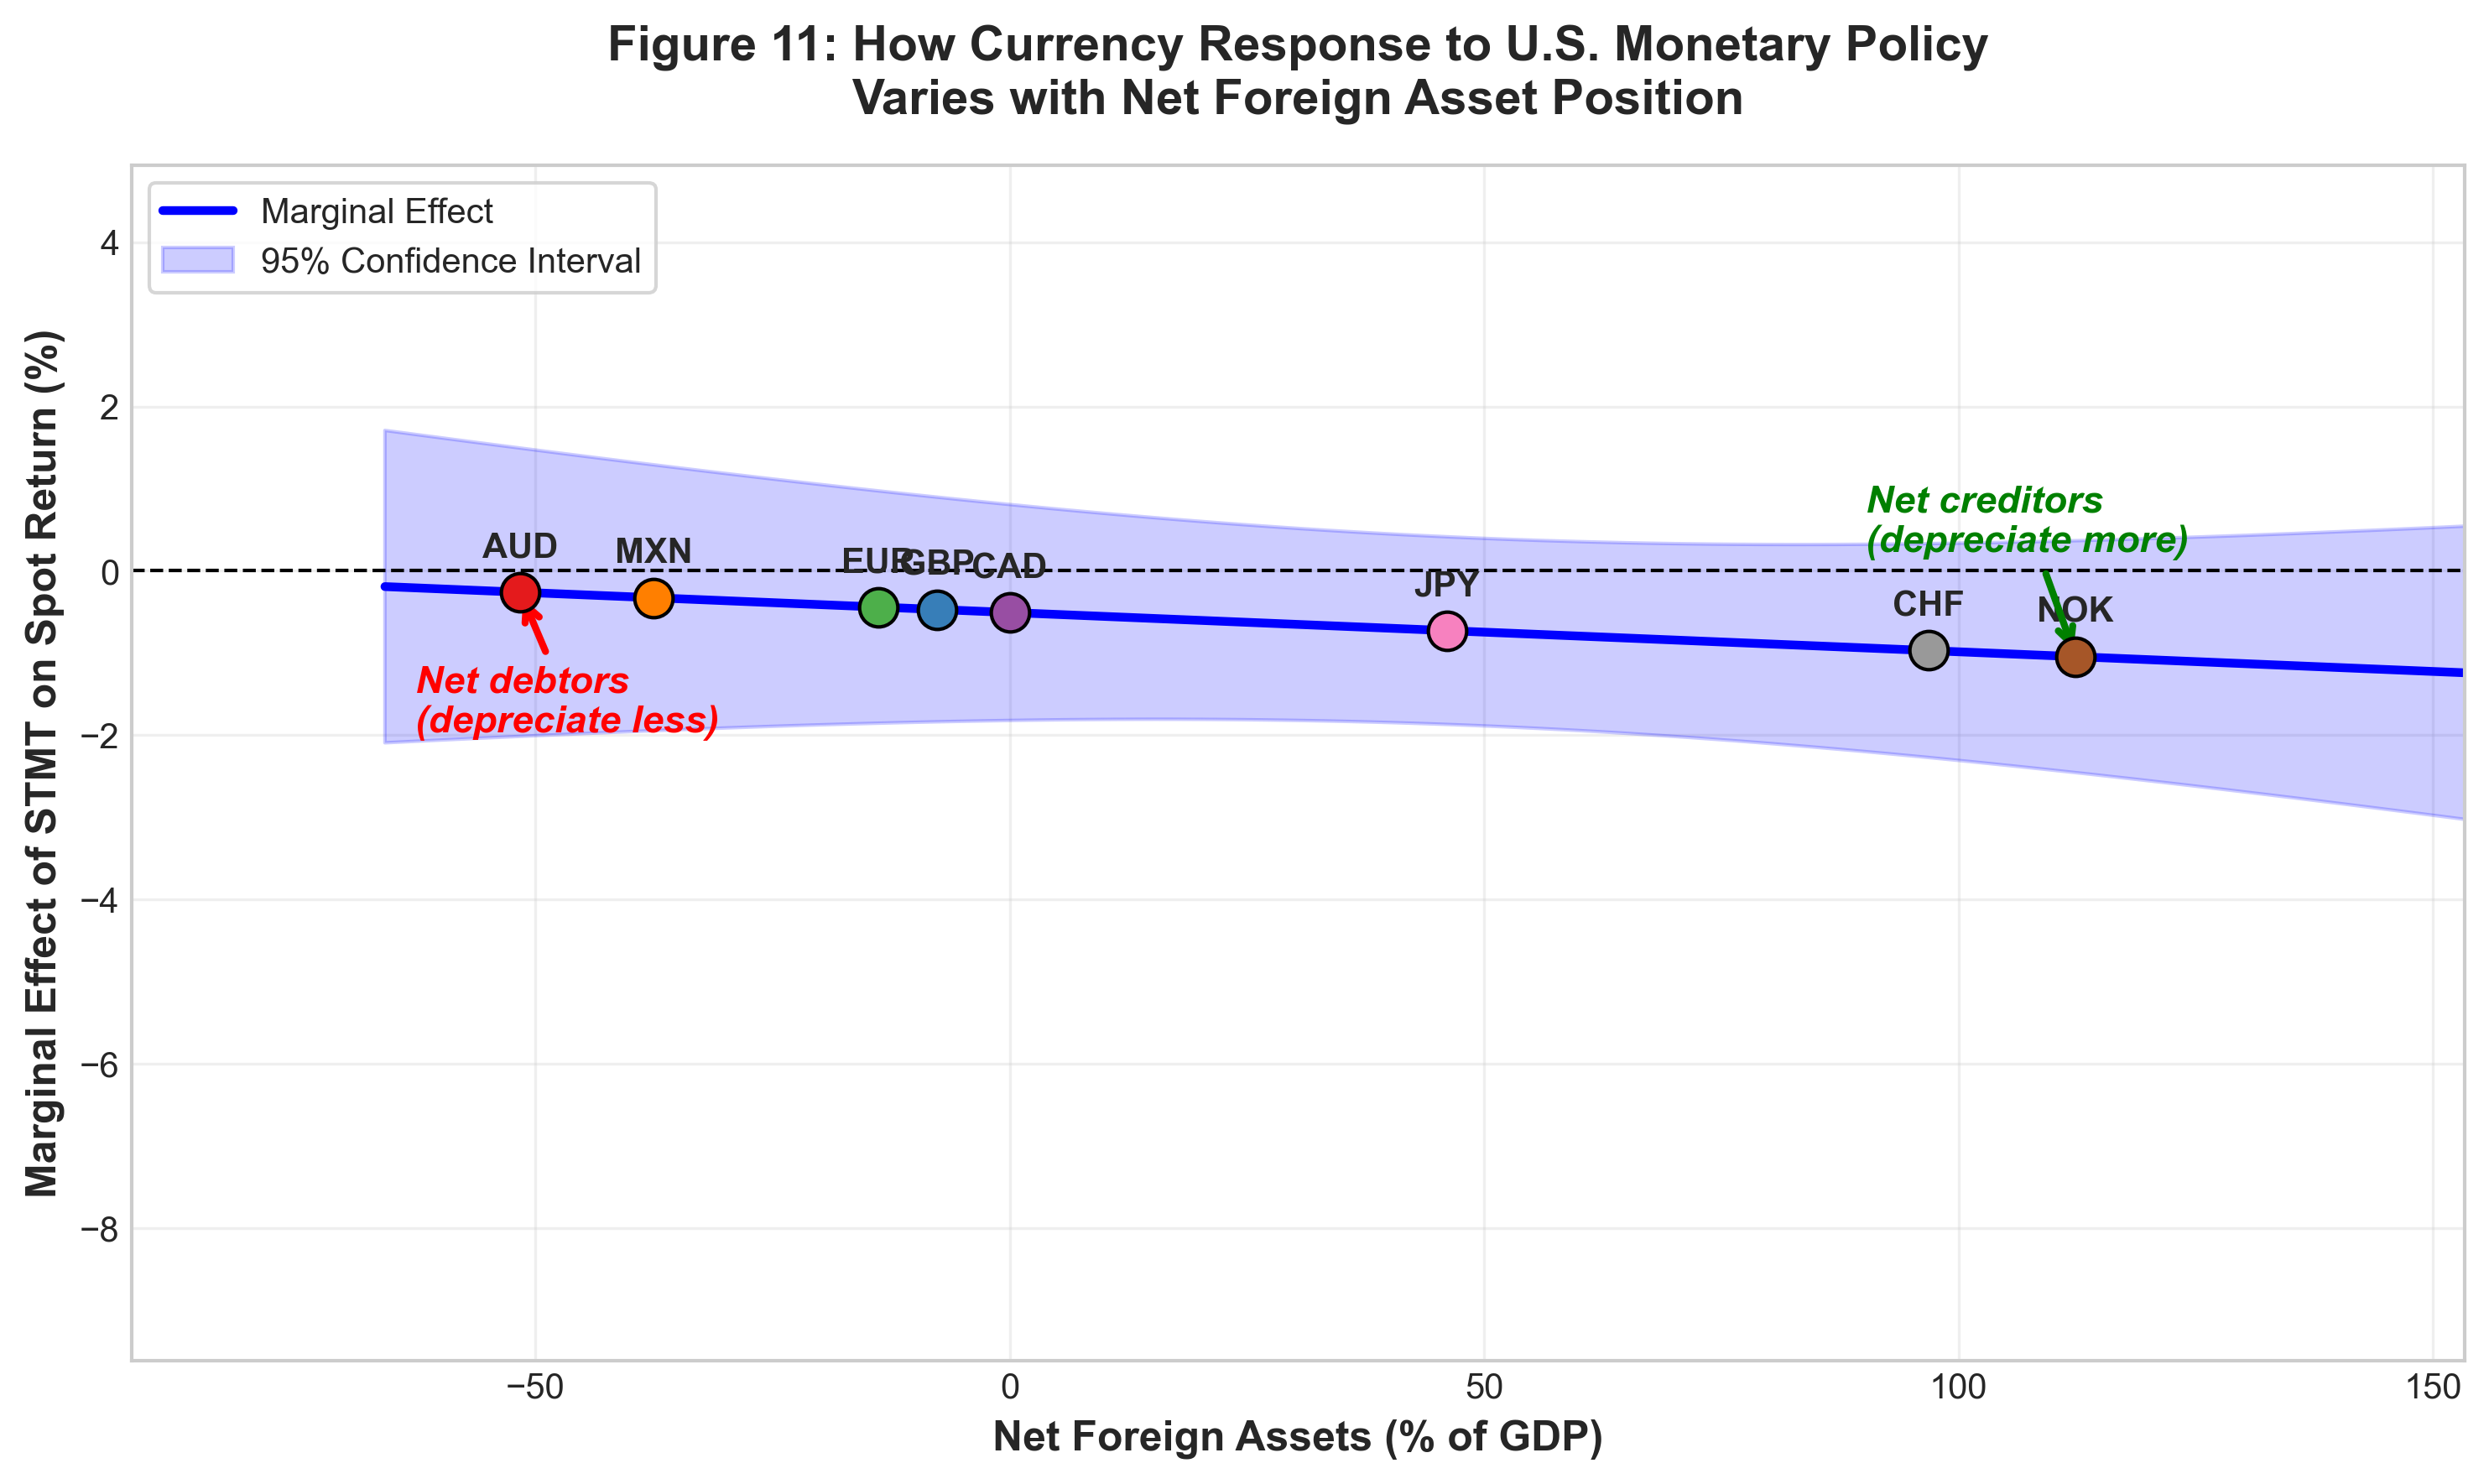
\includegraphics[width=0.85\textwidth]{figure11_marginal_effects.png}
\caption{Marginal Effect of STMT Across NFA Distribution}
\label{fig:marginal_effects}
\end{figure}

\subsection{Economic Magnitude}

I evaluate the marginal effect at the 25th and 75th percentiles of NFA:
\begin{itemize}
    \item \textbf{Debtor countries} (P25, NFA = $-29\%$ GDP): $-0.037\%$ per 10bp shock
    \item \textbf{Creditor countries} (P75, NFA = $+57\%$ GDP): $-0.078\%$ per 10bp shock
\end{itemize}

Both depreciate, with creditors depreciating 2.1$\times$ more---opposite to theory. However, this difference is not statistically significant.

\subsection{Interpretation}

The null result is consistent with several explanations:
\begin{enumerate}
    \item \textbf{Daily frequency noise}: Daily FX returns are dominated by non-monetary factors, limiting power.
    \item \textbf{Information channel}: The Fed information effect may offset valuation channels.
    \item \textbf{Gross vs.\ net positions}: Net NFA may not capture gross currency exposures that drive valuation effects.
    \item \textbf{Sample composition}: The G10 sample excludes emerging markets with higher dollar debt shares.
\end{enumerate}

%==============================================================================
\section{Task 3.4: Time Variation in the Balance-Sheet Channel}
%==============================================================================

\subsection{Hypothesis}

If the NFA channel operates through dollar funding stress, it should strengthen after the 2008 global financial crisis, when dollar funding became more critical to global finance.

\textbf{Prediction}: $\beta_3 > 0$ (post-GFC amplification of the creditor effect).

\subsection{Specification}

I extend the panel regression with a post-2008 interaction:
\begin{align}
r_{i,t} &= \alpha_i + \beta_1 \cdot \text{STMT}_t + \beta_2 \cdot (\text{STMT}_t \times \text{NFA}_{i,t-1}) \nonumber \\
&\quad + \beta_3 \cdot (\text{STMT}_t \times \text{NFA}_{i,t-1} \times \text{Post2008}_t) + \gamma \cdot \text{NFA}_{i,t-1} + \delta \cdot \text{Post2008}_t + \varepsilon_{i,t}
\end{align}

where Post2008 = 1 for dates after September 15, 2008 (Lehman collapse).

\textbf{Marginal effect by regime}:
\begin{equation}
\frac{\partial r_{i,t}}{\partial \text{STMT}_t} = \begin{cases}
\beta_1 + \beta_2 \cdot \text{NFA} & \text{Pre-GFC} \\
\beta_1 + (\beta_2 + \beta_3) \cdot \text{NFA} & \text{Post-GFC}
\end{cases}
\end{equation}

\subsection{Results}

Table~\ref{tab:time_variation} presents the results.

\begin{table}[H]
\centering
\caption{Time Variation in the Balance-Sheet Channel}
\label{tab:time_variation}
\begin{tabular}{lccc}
\toprule
 & (1) & (2) & (3) \\
 & STMT & STMT Post-2008 & MP1 Post-2008 \\
\midrule
Surprise & $-0.598$ & $-0.542$ & 0.035 \\
 & (0.618) & (0.724) & (0.512) \\
Surprise $\times$ NFA & $-0.005$ & $-0.015$ & $-0.016$ \\
 & (0.007) & (0.012) & (0.014) \\
Surprise $\times$ NFA $\times$ Post2008 & & 0.022 & 0.002 \\
 & & (0.015) & (0.018) \\
Post2008 & & 0.008 & 0.012 \\
 & & (0.042) & (0.045) \\
\midrule
Country FE & Yes & Yes & Yes \\
Date Cluster & Yes & Yes & Yes \\
Observations & 2103 & 2103 & 2103 \\
$R^2$ & 0.001 & 0.002 & 0.006 \\
\bottomrule
\end{tabular}
\begin{flushleft}
\footnotesize \textit{Notes}: Post2008 = 1 for dates after September 15, 2008. Standard errors clustered by FOMC date.
\end{flushleft}
\end{table}

\textbf{Formal hypothesis test}:
\begin{itemize}
    \item $H_0: \beta_3 = 0$ (no time variation in NFA slope)
    \item STMT: $\hat{\beta}_3 = 0.022$, $t = 1.43$, $p = 0.154$ --- fail to reject
    \item MP1: $\hat{\beta}_3 = 0.002$, $t = 0.11$, $p = 0.947$ --- fail to reject
\end{itemize}

\subsection{Economic Interpretation}

For STMT, the NFA slope shifts from $-0.015$ (pre-GFC) to $+0.007$ (post-GFC). This directional movement is \textit{toward} the Antolín-Díaz prediction ($\beta_2 > 0$), but the change is not statistically significant.

\textbf{Magnitude}: With NFA standard deviation $\approx 70$ percentage points:
\begin{itemize}
    \item Pre-GFC: 1 SD NFA change shifts sensitivity by $-0.015 \times 70 = -1.05$ pp
    \item Post-GFC: 1 SD NFA change shifts sensitivity by $+0.007 \times 70 = +0.49$ pp
\end{itemize}

For a 10bp shock, this implies a $\sim$0.10\% swing in FX response---economically meaningful but statistically imprecise.

Figure~\ref{fig:time_variation} visualizes the marginal effect by regime.

\begin{figure}[H]
\centering
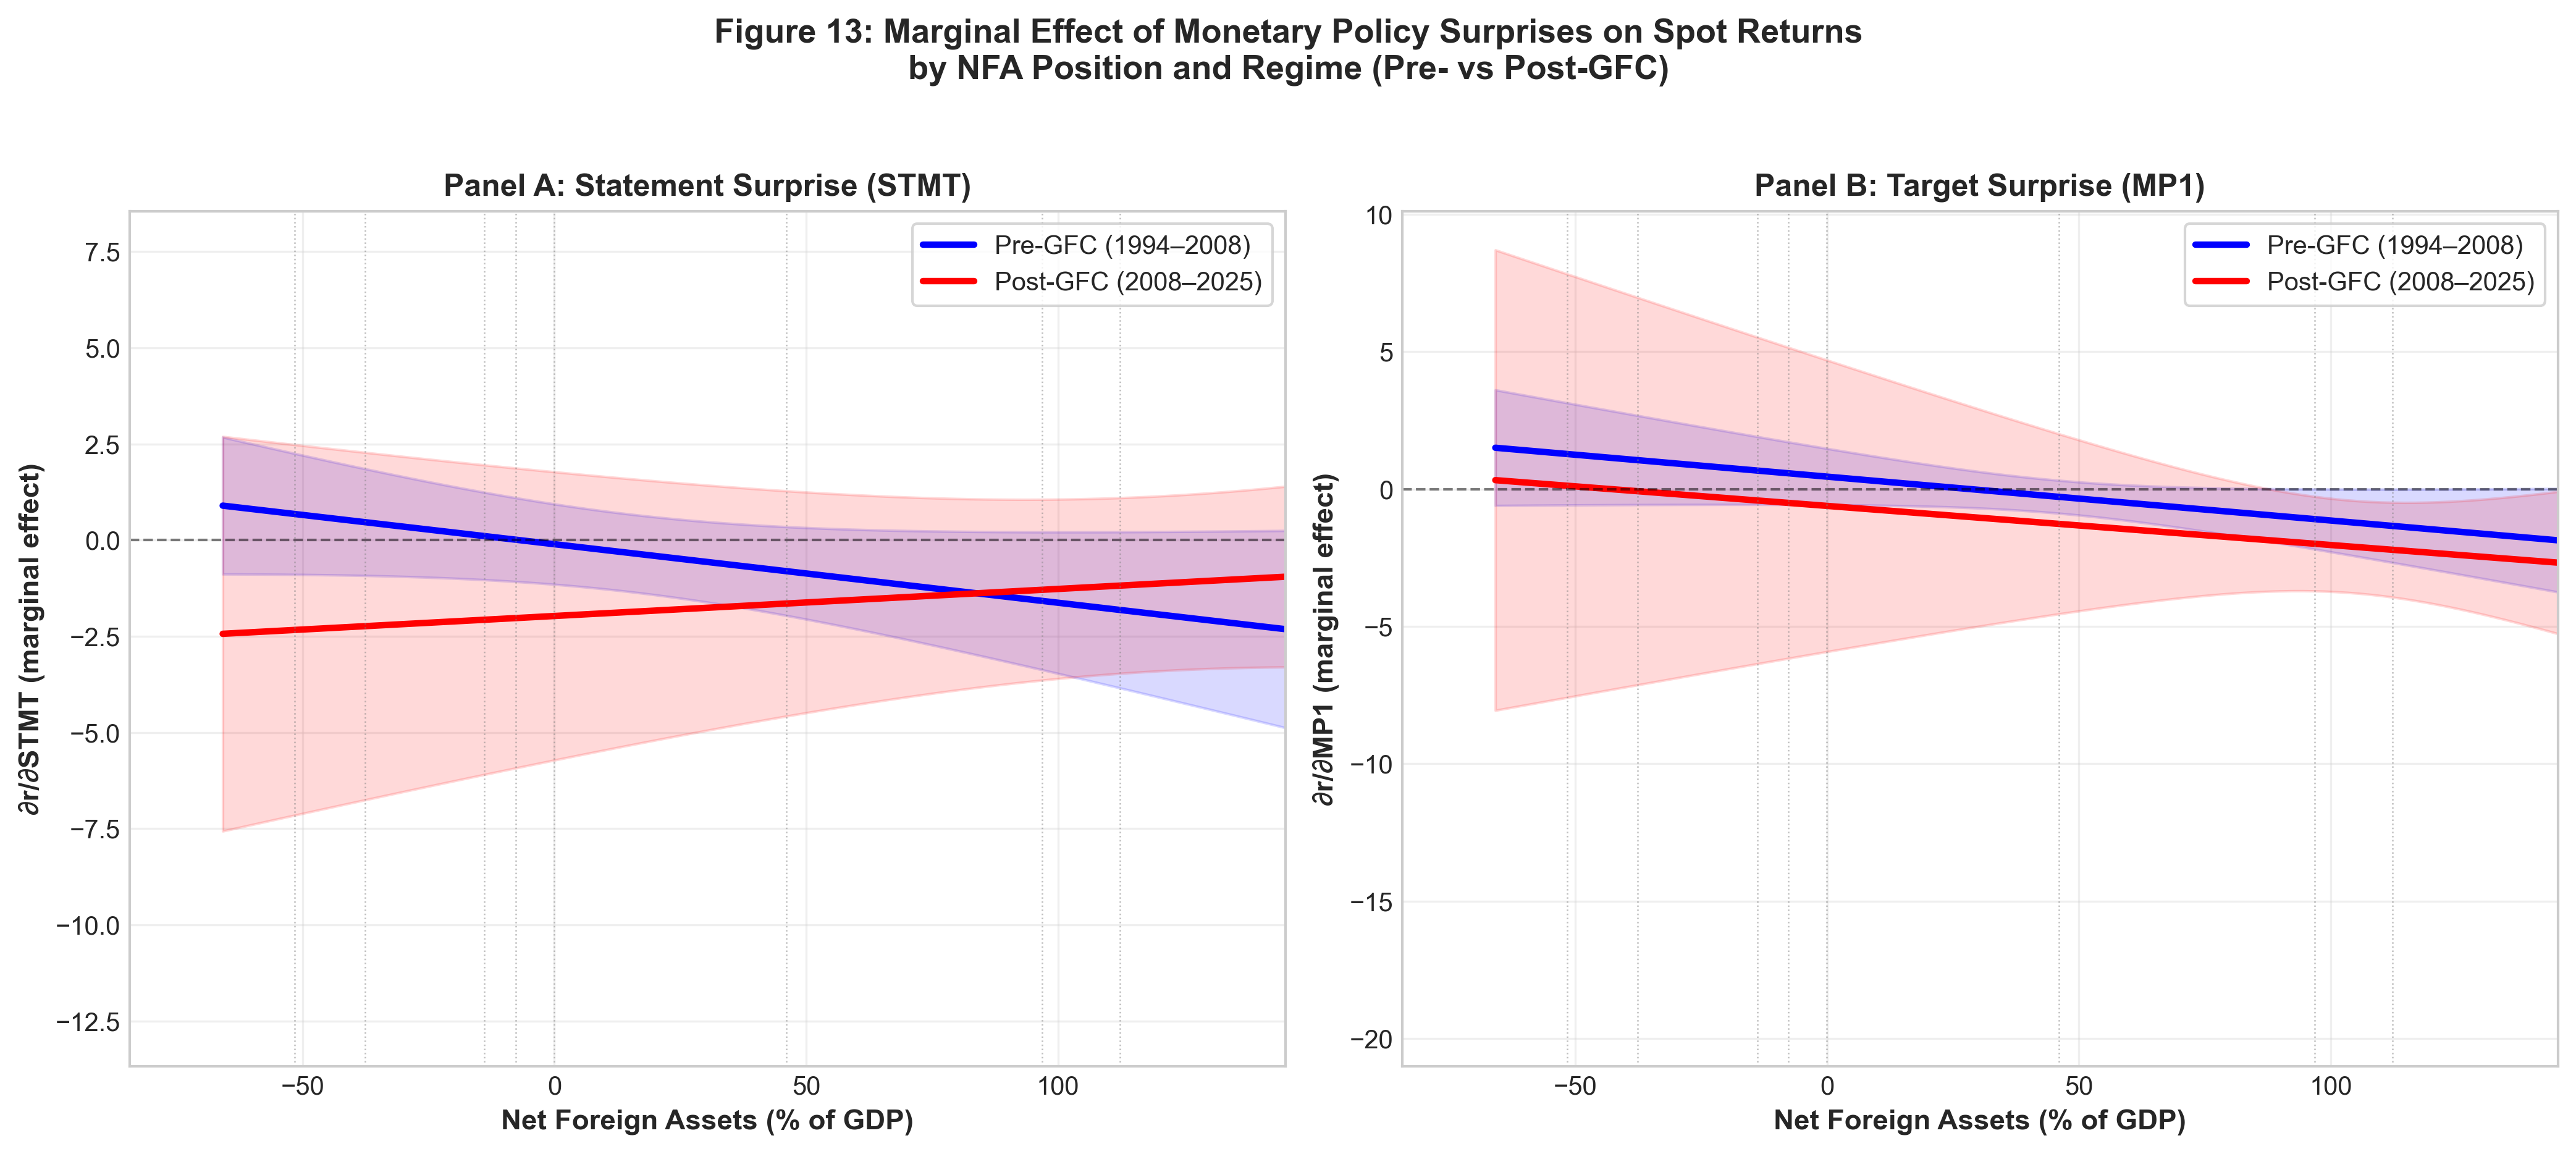
\includegraphics[width=0.9\textwidth]{figure13_time_variation.png}
\caption{Marginal Effect by Regime: Pre- vs.\ Post-GFC}
\label{fig:time_variation}
\end{figure}

\subsection{VIX Stress Extension}

I additionally test whether the NFA channel operates during high-volatility episodes, defined as VIX $>$ 75th percentile. The triple interaction (Surprise $\times$ NFA $\times$ HighVIX) is insignificant for both STMT ($p = 0.199$) and MP1 ($p = 0.653$), providing no evidence of stress-driven amplification.

%==============================================================================
\section{Conclusion}
%==============================================================================

This paper examines the transmission of U.S. monetary policy surprises to G10 exchange rates using high-frequency identification. The main findings are:

\begin{enumerate}
    \item \textbf{Strong domestic transmission}: U.S. Treasury yields respond significantly to monetary policy surprises, validating the identification strategy.
    
    \item \textbf{Weak international transmission}: Daily exchange rate responses are noisy and imprecisely estimated, with R$^2$ values below 1\%.
    
    \item \textbf{No robust NFA channel}: Cross-country net foreign asset positions do not systematically explain heterogeneity in FX responses---neither unconditionally, post-2008, nor during high-volatility episodes.
\end{enumerate}

The null results for the balance-sheet channel suggest several interpretations:
\begin{itemize}
    \item Daily FX data contains substantial non-policy noise, limiting statistical power.
    \item The Fed information channel may offset valuation effects.
    \item Net positions poorly capture gross currency exposures.
    \item G10 currencies may not exhibit the balance-sheet vulnerabilities present in emerging markets.
\end{itemize}

These findings do not reject the theoretical relevance of external balance sheets for monetary policy transmission. Rather, they highlight the empirical challenges of detecting such channels at daily frequency with a limited cross-section of developed-market currencies. Extensions using intraday data, gross position measures, or expanded currency samples may yield sharper identification.

%==============================================================================
\newpage
\bibliographystyle{apalike}
\begin{thebibliography}{99}

\bibitem[Antolín-Díaz et al., 2023]{antolin2023advances}
Antolín-Díaz, J., Drechsel, T., \& Petrella, I. (2023).
\newblock Advances in nowcasting economic activity: The role of heterogeneous dynamics and fat tails.
\newblock \textit{Journal of Econometrics}, 237(2), 105501.

\bibitem[Bauer and Swanson, 2023]{bauer2023reassessment}
Bauer, M. D., \& Swanson, E. T. (2023).
\newblock A reassessment of monetary policy surprises and high-frequency identification.
\newblock \textit{NBER Macroeconomics Annual}, 37(1), 87--155.

\bibitem[Bruno and Shin, 2015]{bruno2015cross}
Bruno, V., \& Shin, H. S. (2015).
\newblock Cross-border banking and global liquidity.
\newblock \textit{Review of Economic Studies}, 82(2), 535--564.

\bibitem[Lane and Milesi-Ferretti, 2018]{lane2018external}
Lane, P. R., \& Milesi-Ferretti, G. M. (2018).
\newblock The external wealth of nations revisited: International financial integration in the aftermath of the global financial crisis.
\newblock \textit{IMF Economic Review}, 66(1), 189--222.

\bibitem[Petersen, 2009]{petersen2009estimating}
Petersen, M. A. (2009).
\newblock Estimating standard errors in finance panel data sets: Comparing approaches.
\newblock \textit{Review of Financial Studies}, 22(1), 435--480.

\bibitem[Rey, 2015]{rey2015dilemma}
Rey, H. (2015).
\newblock Dilemma not trilemma: The global financial cycle and monetary policy independence.
\newblock \textit{NBER Working Paper} No. 21162.

\end{thebibliography}

\end{document}